
\chapter{Application for controlling a robot via SSVEP}
\label{sec:SSVEP_BCI}

The aim of this chapter is to describe the \gls{SSVEP}-based \gls{BCI} designed as a practical part of this thesis. The \gls{BCI} is written in Python 2.7 and the code is accessible from Github repository\footnote{github.com/kahvel/VEP-BCI}. In addition to the Python 2.7 standard library, the following libraries were used:
\begin{itemize}
	\item Emokit\footnote{https://github.com/openyou/emokit/tree/master/python/emokit} to access raw data from Emotiv EPOC headset;
	\item PsychoPy~\cite{psychopy} for designing visual stimuli and precise timing of the stimuli presentations;
	\item scikit-learn~\cite{scikit-learn} for calculating \gls{CCA} algorithm;
	\item SciPy and NumPy~\cite{scipy} for calculating other advanced mathematical algorithms, for example \gls{FFT};
	\item PyQtGraph\footnote{http://www.pyqtgraph.org} for real-time plotting of the data.
\end{itemize} The \gls{BCI} requires only Emotiv EPOC headset and a computer, no specific hardware like digital signal processors or \glspl{LED} are used.

\section{Related work}

There are many types of \glspl{BCI} available. A review by Bashashati \textit{et al.}~\cite{bci_comparison} contains a detailed overview of \gls{EEG}-based \glspl{BCI}. Their paper includes overview of the following neuromechanisms used in \gls{EEG}-based \glspl{BCI}: \gls{VEP} and \gls{SSVEP}, P300, slow cortical potential, response to mental task, sensorimotor activity, and multiple neuromechanisms or hybrid \gls{BCI}. Hybrid \gls{BCI} uses at least two different neuromechanisms in a \gls{BCI} and therefore at least two different methods are required to analyse the \gls{EEG} recording~\cite{hybrid_bci, hybrid_bci2}.

\gls{SSVEP}-based \glspl{BCI} can be divided in categories according to the method used to detect \glspl{SSVEP} in \gls{EEG} recording. Current \gls{SSVEP}-based \gls{BCI} \gls{feature extraction} methods include:
\begin{itemize}
	\item \Gls{PSDA} method introduced by Cheng \textit{et al.}~\cite{psda}.
	\item \Gls{SC} method introduced by Wu and Yao~\cite{sc}.
	\item Dual-frequency \gls{SSVEP} methods~\cite{dual1, dual2}.
	\item \Gls{MPCC} method introduced by Tong \textit{et al.}~\cite{MPCC}.
	\item \Gls{MEC} method introduced by Friman \textit{et al.}~\cite{mec}. This method has shown better performance than \gls{SC} and \gls{PSDA} method~\cite{mec_comparison}.
	\item \Gls{CCA} method introduced by Lin \textit{et al.}~\cite{cca_lin}. This method has shown better performance than \gls{PSDA} method~\cite{cca_psda, bin2009cca, cca_lin}.
	\item Multiway \gls{CCA} method introduced by Zhang \textit{et al.}~\cite{mcca}. This method has shown better performance than standard \gls{CCA}~\cite{mcca}.
	\item \Gls{LASSO} method introduced by Zhang \textit{et al.}~\cite{LASSO}. This method has shown better performance than \gls{CCA} method~\cite{LASSO}.
	\item \Gls{LRT} method introduced by Zhang \textit{et al.}~\cite{LRT}. This method has shown better performance than \gls{CCA} method and similar performance to \gls{LASSO} method~\cite{LRT}.
\end{itemize}
For more comprehensive review of the \gls{feature extraction} methods see article by Liu \textit{et al.}~\cite{feature_extraction}.

In this thesis, Emotiv EPOC is used to record brain activity. Table~\ref{tab:emotiv_BCIs} gives overview of the existing \glspl{BCI} that also use Emotiv EPOC for recording brain activity. It can be seen that existing applications have \gls{target} detection time above or exactly three seconds which is not fast enough to control a robot in real time. However, as Zier mentioned in his paper~\cite{emotiv_psda} and as also noticed in the process of developing this application, if the \gls{window} length is long enough for the \gls{feature extraction} method to accurately detect correct \gls{target}, the \gls{target} detection time is about half the \gls{window} length. That is so, because after half the \gls{window} length, half of the previous data is replaced with new data and if there is more new data than previous, then the \gls{BCI} recognises the new user's choice.

\newcommand{\liu}{Liu \textit{et al.}~\cite{emotiv_11hz}}
\newcommand{\lin}{Lin \textit{et al.}~\cite{emotiv_walking}}
\newcommand{\choi}{Choi and Jo~\cite{emotiv_hybrid}}
%\newcommand{\zier}{Zier~\cite{emotiv_psda}}
\newcommand{\hvar}{Hvaring and}
\newcommand{\moe}{Ulltveit-Moe~\cite{emotiv_comparison}}
\newcommand{\duvi}{Duvinage \textit{et al.}~\cite{emotiv_p300_comp}}

\begin{table}[h]
	\centering
	\begin{tabular}{|c|c|c|c|c|}\hline
		& Method& Accuracy (\%)		& Target detection 	& ITR (bits/min)	\\
		&		&					& time (sec)		&					\\\hline
\liu	& CCA	& $95.83\pm 3.59$	& $5.25\pm 2.14$	& $20.97\pm 0.37$	\\\hline
\lin	& CCA	& $76.60\pm 21.74$	& $4.34\pm 0.08$	& $14.38\pm 9.04$	\\\hline
		& CCA	& $84.4\pm 5.0$		& N/A				& $11.6\pm 3.9$		\\\cline{2-5}
\choi	& ERD	& $84.6\pm 5.3$		& N/A				& $11.8\pm 3.7$		\\\cline{2-5}
		& P300	& $89.5$			& $5.35$			& $18.1\pm 2.1$		\\\hline
\hvar	& CCA	& $85.12\pm 4.58$	& $3.00$			& $32.92\pm 4.72$	\\\cline{2-5}
\moe	& PSDA	& $89.29\pm 6.41$	& $5.14\pm 0.98$	& $23.78\pm 7.15$	\\\hline
	\end{tabular}
	\caption{Comparison of the existing BCIs that use Emotiv EPOC.}
	\label{tab:emotiv_BCIs}
\end{table}

This thesis aims at developing \gls{BCI} with faster \gls{target} detection time than the previous applications to provide suitable speed for controlling a robot.
%This thesis focuses on two of these methods: \gls{PSDA} and \gls{CCA} methods.

\section{Using the application with other EEG devices}
\label{sec:different_devices}

Although the application was written for Emotiv EPOC, it can be used with other \gls{EEG} devices too if it is possible to access the data of these devices with Python script. The communication between the data accessing code and the rest of the application is realised using Python multiprocessing module. The data accessing code runs on separate process and communicates with the rest of the application by sending messages through multiprocessing connection. It sends raw data through the connection and receives messages like "Setup", "Start", "Stop" and "Exit". Each of the received messages should lead to calling a specific function. If the received message is
\begin{itemize}
	\item "Setup", then the object should get internally ready to start sending data;
	\item "Start", then the object should start sending the data;
	\item "Stop", then the object should stop sending the data;
	\item "Exit", then all the needed clean up procedures should be executed, because the application is closing.
\end{itemize}

The easiest way to start using different headset with the application is changing the code in MyEmotiv.py. The constructor of MyEmotiv class has to take one argument. This argument is the object that handles the communication between different processes. The last line in the constructor of MyEmotiv should call the argument's waitMessages method, which waits until it receives one of the previously discussed messages. The waitMessages method takes arguments which are the functions that are called when corresponding message is received. By replacing these methods in MyEmotiv object, it is possible to use the application with other \gls{EEG} devices too. Since the application can be relatively easily modified to use other \gls{EEG} devices too, it could be a good tool to test how suitable are different devices for a \gls{SSVEP}-based \gls{BCI}.

\section{Signal pipeline of the application}
\label{sec:signal_pipeline}

The application does not have one specific signal pipeline, but the components of the pipeline can be changed using the graphical user interface. This allows different configurations to be easily tested to find the best settings for controlling a robot and the best settings for different users.

\begin{figure}[h!]
	\tikzstyle{decision} = [diamond, draw, fill=blue!20,
    text width=4.5em, text badly centered, node distance=2.5cm, inner sep=0pt]
\tikzstyle{block} = [rectangle, draw, fill=blue!20,
    text width=5em, text centered, rounded corners, minimum height=4em]
\tikzstyle{line} = [draw, very thick, color=black!50, -latex']
\tikzstyle{cloud} = [draw, ellipse,fill=red!20, node distance=3cm,
    minimum height=2em]

\begin{tikzpicture}[scale=2, node distance = 4cm, auto]
	% Nodes
	\node [cloud] (start) {start};
	\node [decision, below of=start] (wait) {wait for step packets};
	\node [block, right of=wait] (filter) {filter new signal segment};
	\node [cloud, right of=start] (stop) {stop};
	\node [block, right of=filter] (add) {add segment to signal};
	\node [decision, right of=add, node distance=4 cm] (length) {len(signal) \textgreater window length?};
	\node [block, below of=length] (delete) {delete first step packets};
	\node [block, left of=delete] (detrend) {make copy of signal and detrend it};
	\node [block, left of=detrend] (window) {window signal};
	\node [block, left of=window] (detect) {send signal to feature extraction};
	
	% Arrows
	\path [line] (start) -- (wait);
	\path [line] (wait) -- node [align=center, color=black, sloped, pos=1] {received\\"Stop"} (stop);
	\path [line] (wait) -- node [align=center, color=black, sloped] {received\\data} (filter);
	\path [line] (filter) -- (add);
	\path [line] (add) -- (length);
	\path [line] (length) -- node [near start, color=black] {yes} (delete);
	\path [line] (length) -- node [near start, color=black] {no} (detrend);
	\path [line] (detrend) -- (window);
	\path [line] (delete) -- (detrend);
	\path [line] (window) -- (detect);
	\path [line] (detect) -- (wait);
\end{tikzpicture}

	\caption{Flowchart of the application's signal pipeline.}
	\label{fig:signal_pipeline}
\end{figure}

All the signal processing techniques discussed in section~\ref{sec:signal_processing} can be used as components of the signal pipeline. In addition to these components, filtering can also be used. See figure~\ref{fig:options_frame} for illustration of the application's user interface for choosing signal pipeline components and options.

\begin{figure}[h]
	\centering
	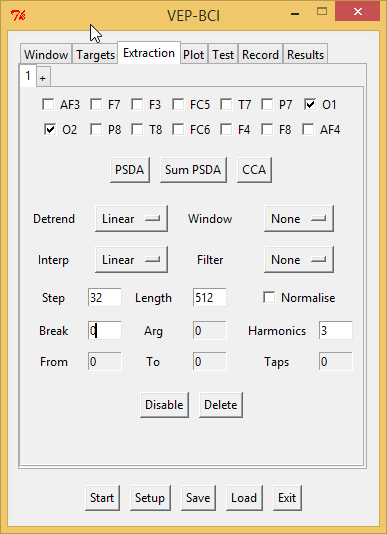
\includegraphics[width=0.6\textwidth]{options_frame.png}
	\caption{The user interface for choosing signal pipeline options.}
	\label{fig:options_frame}
\end{figure}

The explanation of the signal pipeline options is the following:
\begin{enumerate}
	\item \Gls{detrend} is either linear, constant or none. None means that \glsdisp{detrend}{detrending} is not used. Linear means that linear trend is removed from the raw signal; constant means that constant trend is removed from the raw signal. \glsdisp{detrend}{Detrending} is more thoroughly discussed in section~\ref{sec:detrend}.
	\item \Gls{window} is either hann, hamming, blackman, keiser, bartlett or none. None means that \gls{window} function is not used. Other options are standard signal processing \gls{window} functions. \glsdisp{window}{Windowing} is more thoroughly discussed in section~\ref{sec:window}.
	\item \glsdisp{interpolation}{Interp} is either linear, nearest, zero, slinear, quadratic or cubic. See SciPy documentation\footnote{https://docs.scipy.org/doc/scipy/reference/generated/scipy.interpolate.interp1d.html\#scipy.interpolate.interp1d} for more information. \Gls{interpolation} is more thoroughly discussed in section~\ref{sec:interpolate}.
	\item Filter is either high-pass, low-pass, band-pass or none. None means that filtering is not used. High-pass filter means that frequencies lower than the given value are removed from the signal. Similarly, low-pass filter removes frequencies higher than the given value. Band-pass filter takes two values and removes frequencies that are not in the given range. See SciPy documentation\footnote{\label{firwin}http://docs.scipy.org/doc/scipy/reference/generated/scipy.signal.firwin.html\#scipy.signal.firwin} for more information. 
	\item Step shows how many packets have to be received before trying to identify user's choice. For example, if \gls{sampling rate} is \SI{128}{Hz} and step is 64 then the \gls{feature extraction} algorithms are executed after every $\frac{64}{\SI{128}{Hz}}=0.5$ seconds.
	\item Length is the length of the window. Length shows the number of packets on which the \gls{feature extraction} algorithms are executed. For example, if \gls{sampling rate} is \SI{128}{Hz} and length is 512 then the \gls{feature extraction} algorithms are performed on the last $\frac{512}{\SI{128}{Hz}}=4$ seconds of data.
	\item Break is the number of breakpoints used when \glsdisp{detrend}{detrending} the signal. The breakpoints will be equally spaced. If the number of breakpoints is 1, then the breakpoint will be in the middle of the signal and the trend will be removed separately from the first half of the signal and the second half of the signal.
	\item Arg is the beta argument for kaiser window. See NumPy documentation for details\footnote{http://docs.scipy.org/doc/numpy/reference/generated/numpy.kaiser.html}.
	\item Harmonics is the number of integer multiples used in \gls{feature extraction} methods. How integer multiples of the \gls{target} frequency can be used in \gls{PSDA} and \gls{CCA} extraction methods was discussed in sections~\ref{sec:PSDA} and \ref{sec:CCA} respectively. The motivation for using integer multiples was discussed in section~\ref{sec:decomposition}.
	\item Normalise shows whether to normalise the estimated \gls{power spectral density} as in equation~\ref{eq:norm_SNR} or not.
	\item From and to are the frequencies used to specify the filter arguments. From shows the lowest frequency that is passed, smaller frequencies will be removed; to shows the highest frequency that is passed, lower frequencies are removed.
	\item Taps shows the number of taps or the length of the filter. See SciPy documentation\addtocounter{footnote}{-2}\footnotemark\addtocounter{footnote}{1} for details.
\end{enumerate}

One thing to keep in mind is that the window length shows how many unprocessed packets are held in the memory. This means that after every step, the whole signal goes through the signal pipeline, not only the segment obtained during the last step.

The application has graphical user interface and the code is written so that it is relatively easy to add new or change the existing functionality, as briefly discussed in section~\ref{sec:different_devices}. Thus this application can be used to compare how different signal pipelines affect the detection of \glspl{SSVEP}.

\section{Target identification method}
\label{sec:identification}

This section describes the user's choice identification method used in this application. To the best of the author's knowledge, this \gls{target} identification method has not been used before. As is the case with the signal pipeline, this application actually does not have one specific \gls{feature extraction} method, but the \gls{feature extraction} method can be changed and a combinations of different \gls{feature extraction} methods can be used.

Currently the application has three different \gls{feature extraction} methods that can be combined: widely known \gls{PSDA} and \gls{CCA} method and a method that is similar to the \gls{PSDA} method but the estimated \gls{power spectral density} is calculated not for each signal obtained from different channels but for the sum of all the signals from different channels. If only one channel is used, then this method works exactly the same as standard \gls{PSDA} method. In the graphical user interface, this method is called sum \gls{PSDA} method. Using this method makes sense, because \gls{FFT} is linear, meaning that the result will be the same if first the signals are summed up and then the \gls{power spectral density} is estimated and if first the \gls{power spectral density} is estimated separately for each channel and then the \gls{power spectral density} estimates for each channel are summed up.

The standard \gls{PSDA} method gives separate results for each channel. One way to identify user's choice is to choose a command if all the separate results are the same, meaning that the \gls{PSDA} method gave same result for all the used channels. Similarly, to the \gls{PSDA} method \gls{target} identification

All \gls{feature extraction} methods used in the application can be combined. In case of combining methods, the \gls{target} choosing procedure is similar to the standard \gls{PSDA} method---all the methods have to give the same result. Currently this can not be changed from the user interface. If different \gls{target} choosing method is needed, then the code has to be changed. This functionality can easily be changed, when changing the code in PostOffice.py in handleFreqMessage method. This method receives results through a connection similarly to the data accessing code discussed in section~\ref{sec:different_devices}. The results have already been organised into different data structures. There are results per each method, results per each signal pipeline, all the results counted and other data structures to make it easier to further develop the application.

It is also worth mentioning that different methods can have different signal pipelines. For example it would not make sense to \gls{window} a signal that is later analysed using \gls{CCA}, but it could be beneficial if the estimated \gls{power spectral density} of the signal is later analysed using \gls{PSDA} method. Thus the application has the functionality to use signal pipelines with different options, which gives even more flexibility.

Using \gls{PSDA} and \gls{CCA} method together makes the \gls{target} identification more accurate, since different methods have to give the same result. If one of the methods makes a mistake and gives the wrong result, then the other method might still give the correct result. It is more probable for one method to make mistake than two methods at the same time. These two method analyse the \gls{EEG} signal from two different aspects---one uses time-domain representation, the other uses frequency-domain representation.

To further improve this method, the phase information from the \gls{frequency spectrum} that is currently being discarded could also be used. One possible usage would be to design \gls{CCA} method \glspl{reference signal} with correct phase. Currently both sine and cosine waves are used to achieve optimal minimum correlation as discussed in section~\ref{sec:CCA}.

\section{Controlling the robot with the application}

As discussed in section~\ref{sec:identification}, the application does not have one specific \gls{feature extraction} method but it combines different \gls{feature extraction} methods with different signal pipelines if necessary. Thus the way how the signal is processed and how the user's choice is identified is modifiable. This section describes how the command that the user chose is used to control a robot. See figure~\ref{fig:robot} for a picture of the robot used for testing the application.

\begin{figure}[h]
	\centering
	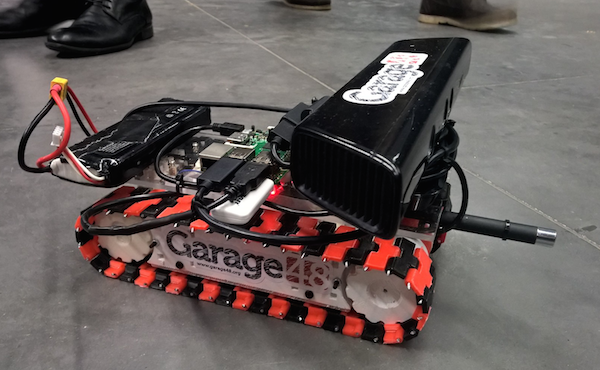
\includegraphics[width=0.6\textwidth]{robot.png}
	\caption{The robot used for testing the application.}
	\label{fig:robot}
\end{figure}

The robot\footnote{https://github.com/kuz/Garage48-PiTank} has five possible commands move forward, move backward, turn left, turn right and stop. The robot can execute one command at a time, meaning that it is not possible to move forward and turn left or right at the same time. If the robot is moving forward and receives different command, the moving forward will stop. The visual stimuli could be designed for example as shown in figure~\ref{fig:arrow_stimuli}.

\begin{figure}[h]
	\centering
	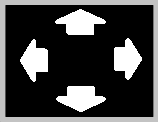
\includegraphics[width=0.4\textwidth]{arrows.png}
	\caption{Stimuli locations on the screen for controlling a robot.}
	\label{fig:arrow_stimuli}
\end{figure}

The robot has a camera on it and thus it is possible to see the videos stream of the camera from the computer screen when controlling the robot with the application. The empty space in the middle of the screen as shown in figure~\ref{fig:arrow_stimuli} is intended---it is possible to show the video stream there.

The communication between the robot and the application is implemented similarly to the communication between other parts of the application, but instead of multiprocessing connections, sockets were used.

[TODO: Add other details of the implementation if needed (not done yet, Ilya is searching for a camera for the robot)].

[TODO: Add the ITR/accuracy/speed and compare to existing BCIs]
